\section{Wykorzystane technologie}
  \subsection{Ruby}
  \label{sec:Ruby}
  \index{Ruby}
  Ruby\footnote{dokumentacja online: \url{http://rubyonrails.org}, \cite{ruby_lang}} jest w pełni obiektowym, wysokopoziomowym językiem programowania. Jego twórca, Yukihiro “Matz” Matsumoto, chciał stworzyć język jeszcze bardziej obiektowy niż Python, dlatego każdy fragment informacji może uzyskać swoje właściwości i metody.

  Po za obiektowością, Ruby cechuje się też prostą składnią, ułożoną w sposób umożliwiający pisanie samo komentującego się i czytelnego kodu. Programiści piszący w tym języku kierują się dwoma ważnymi zasadami: \index{DRY}DRY\footnote{Don't repeat yourself\cite{programming_ruby}} oraz \index{KISS}KISS\footnote{Keep it simple, stupid\cite{programming_ruby}}, które mają za zadanie zmusić do wykorzystywania już wcześniej napisanego kodu jak i pisania go w sposób najmożliwiej prosty. Ponadto, jest to język niezwykle elastyczny, ponieważ pozwala użytkownikom dowolnie modyfikować jego składowe. Programista może nadpisać jakiś moduł i dostosować go do swoich potrzeb.

  Ruby powstał w 1995 roku, lecz dopiero w 2005 roku zyskał na popularności za sprawą frameworka Ruby on Rails, który został w nim napisany. Dzisiaj osoby piszące w Ruby to jedni z najlepiej zarabiających programistów w USA\footnote{\url{http://www.pb.pl/3945225,84037,te-jezyki-programowania-daja-najlepiej-zarobic-w-usa}}.

  \subsection{Ruby on Rails}
  \index{Ruby on Rails}
  \label{sec:Rails}
  Jest to framework, platforma programistyczna, pozwalająca na szybkie tworzenie stron i aplikacji internetowych. Została napisana przez duńskiego programistę Davida Heinemeiera Hanssona, zwanego potocznie DHH. Oparta jest o wzorzec architektoniczny MVC\footnote{Model View Controller, więcej informacji w rozdziale \ref{sec:patterns}}.
  \clearpage
  Tim O'Reilly, założyciel O'Reilly Media, powiedział:
  \begin{quote}
    \emph{,,Ruby on Rails jest przełomem w dziedzinie programowania aplikacji internetowych.
    Potężne aplikacje, których tworzenie do tej pory zabierało tygodnie czy miesiące, są teraz tworzone dosłownie w kilka dni."}, \\
    \small{\textit{żródło: \url{http://www.rubyonrails.pl/}}}
  \end{quote}

  W Ruby on Rails panuje zasada ,,konwencja ponad konfiguracją" (\emph{Convention over configuration}), co znaczy, że nie trzeba się przejmować skomplikowanymi plikami konfiguracyjnymi, tylko wystarczy postępować według przyjętych przez twórców schematów. Railsy mają wbudowany serwer lokalny, co pozwala na szybkie testowanie aplikacji, bez zbędnego i czasochłonnego umieszczania kodu na zewnętrznej maszynie. Dużym plusem jest również możliwość uruchomienia aplikacji w różnym środowisku, do wyboru mamy:
  \begin{itemize}
    \item \textbf{developerskie} - domyślne środowisko, w którym programista pisze aplikację,
    \item \textbf{testowe} - wykorzystywane do testowania aplikacji,
    \item \textbf{produkcyjne} - aplikacja zachowuje się wtedy jakby była już umieszczona na serwerze
  \end{itemize}
  To wszystko sprawia, że klientowi można oddać gotowy, przetestowany produkt, bez żadnych niespodzianek.

  \subsection{Git}
  \index{Git} \label{sec:GIT}
  To rozproszony system kontroli wersji, bardzo pomocny w projektach, przy których pracuje kilka osób. Dzięki niemu widać wszystkie  wcześniej wprowadzane zmiany i w łatwy sposób można wrócić do wcześniejszych wersji. Użytkownik posługuje się tzw. commitami. Jest to nic innego jak zatwierdzenie zmian w plikach. Podobnym narzędziem do Gita jest SVN. Różnica m.in. polega na tym, że Git kopiuje całe repozytorium na komputer, programista zatwierdza zmiany lokalnie i dopiero na koniec wrzuca je na serwer. W przypadku SVN całość trzymana jest na serwerze.
  Dzięki takiemu rozwiązaniu nie musimy być bez przerwy podłączeni do sieci. Możemy zatwierdzać nasze zmiany będąc w autobusie czy tramwaju i wrzucić je na serwer w momencie podłączenia do internetu.
  Różnice między tymi dwoma technologiami pokazuje poniższy obrazek.

  \begin{figure}
    \centering
    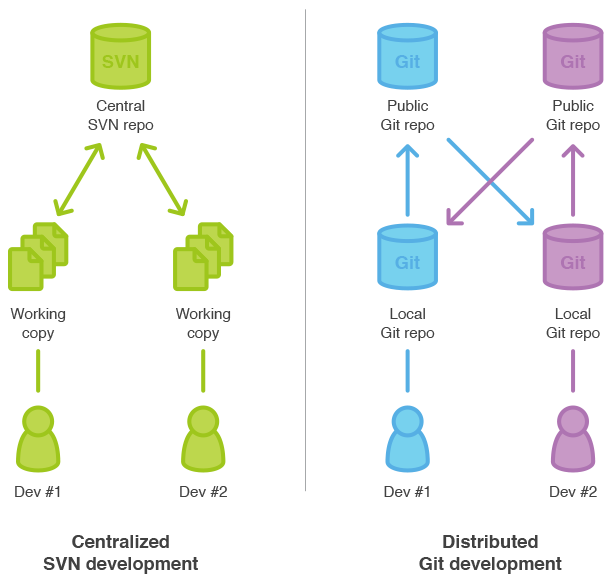
\includegraphics[scale=0.45]{images/gitsvn.png}
    \caption{Różnica w działaniu pomiędzy Git i SVN, \cite{git}}
  \end{figure}

  \subsection{RVM}
  \index{RVM} \label{sec:RVM}
  Czyli \textbf{Ruby Version Manager}\footnote{\url{https://rvm.io/} \cite{programming_ruby}}. Jest to podstawowe narzędzie do pracy z językiem Ruby - zarządza ono jego środowiskiem. Ruby jest ciągle rozwijany i każdego miesiąca wychodzą nowe poprawki, usprawnienia czy funkcjonalności. RVM dla każdego projektu tworzy osobne, niezależne, odizolowane środowisko programistyczne, tzw. gemset. Jest to nic innego jak zbiór gemów wykorzystywanych w danym projekcie. Dzięki temu można stworzyć różne aplikacje oparte o różne wersje Ruby, które korzystają z różnych wersji gemów i nie kolidują ze sobą.
  \begin{figure}[h]
  \centering
  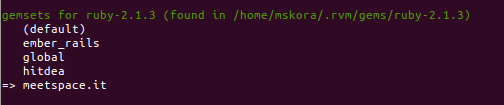
\includegraphics[scale=0.84]{images/rvm.png}
  \caption{Przykładowa lista gemsetów dla Ruby 2.1.3,\cite{rubydoc}}
  \end{figure}

  \subsection{Wykorzystane gemy}
    \index{Gem}
    \textbf{Gem} - jest to paczka napisana w języku Ruby, której zadaniem jest rozszerzenie funkcjonalności aplikacji. Do wyszukiwania najnowszych wersji wykorzystuje się RubyGems.org\footnote{Wyszukiwarka gemów \url{http://rubygems.org}, \cite{rubydoc}}. W przypadku Ruby on Rails istnieje specjalny plik konfiguracyjny, \emph{Gemfile.rb}, który przechowuje listę wykorzystywanych gemów.

    W naszej aplikacji użyliśmy między innymi:
    \begin{itemize}
      \item \textbf{\emph{Devise}} \\ Zapewnia autoryzację i autentykację użytkownika w obrębie aplikacji. Obsługuje logowanie oraz rejestrację wraz z wysyłaniem potwierdzeń na adres mailowy i reset hasła.
      \item \textbf{\emph{Geocoder}} \\ Na podstawie podanego adresu określa współrzędne geograficzne, dzięki którym można wyświetlić mapkę z zaznaczonym adresem, gdzie odbywa się dane wydarzenie.
      \item \textbf{\emph{Omniauth-facebook}} \\ Wspiera komunikację pomiędzy naszą aplikacją a API Facebook'a.
      \item \textbf{\emph{i18n}} \\ Umożliwia dodawanie tłumaczeń, dzięki czemu aplikacja w łatwy sposób może stać się wielojęzyczną.
    \end{itemize}

  \subsection{Narzędzia do testowania}
    Proces testowania jest bardzo ważnym aspektem, przy projektowaniu i tworzeniu oprogramowania. Dzięki Ruby i Ruby on Rails oraz odpowiednim narzędziom jesteśmy w stanie przetestować każdą warstwę aplikacji.

    \begin{itemize}
      \item \textbf{\emph{Cucumber}}\footnote{\cite{cucumber}, \cite{testing_tuesday} } \\
      Wykorzystywany jest do pisania testów funkcjonalnych(\emph{feature tests})\footnote{Szerzej o testach w rozdziale \ref{testy}.}. Tworzony jest krótki scenariusz, w którym krok po kroku sprawdza się czy aplikacja zachowuje się w sposób w jaki oczekuje klient.\index{Cucumber}
      \item \textbf{\emph{RSpec}} \\
      Narzędzie, w którym piszemy testy jednostkowe\footnote{\cite{rspec}, szerzej o testach w rozdziale \ref{testy}}. Pozwala testować nie tylko całą logikę znajdującą się w modelach, relacje między nimi, ale również kontrolery, routy\footnote{RESTowe ścieżki w aplikacji \cite{head_first}}, helpery\footnote{Metody, które pomagają w wyświetlaniu pewnych danych na widoku \cite{rspec},\cite{rails_guide}} oraz wszystkie dodatkowe klasy. \index{RSpec}
    \end{itemize}

  \subsection{Biblioteki JavaScript}
    W aplikacji internetowej JavaScript\cite{java_script} jest nieodłączną częścią, bez której ciężko byłoby wykonać pewne rzeczy. Szczególnie pomaga w ,,upiększaniu" interfejsu aplikacji ale również w komunikacji między przeglądarką a serwerem, jak i wyświetlaniu dodatkowych informacji, na przykład takich jak mapy Google'a.

    \begin{itemize}
      \item \textbf{\emph{jQuery}} \\ \
      Biblioteka JavaScript ułatwiająca manipulację drzewem DOM\footnote{Document Object Model - reprezentacja złożonych dokumentów HTML. \cite{html5_css3}}. Umożliwia tworzenie animacji, wspomaga zarządzanie asynchronicznymi zapytaniami do serwera. Dzięki jej implementacji możliwe jest korzystanie z wielu stworzonych już wtyczek.
      \item \textbf{\emph{Bootstrap Datepicker}} \\
      Oparta o Bootstrap biblioteka, wyświetlająca na stronie ładny i intuicyjny kalendarz.
      \item \textbf{\emph{Load Image}} \\
      Prosta biblioteka umożliwiająca użytkownikowi ładowanie obrazka bezpośrednio na stronie.
      \item \textbf{\emph{Modernizr}} \\
      Przydatna biblioteka, informująca nas, czy dana przeglądarka, obsługuje poszczególne moduły standardu HTML, np. video, canvas czy geolokalizację.
    \end{itemize}
  \subsection{Pozostałe technologie}
    \label{other_technology}
    Poniżej zostały opisane dodatkowe technologie, wykorzystane w aplikacji.
    \begin{itemize}
      \item \textbf{\emph{Twitter Bootstrap}} \\
      Framework CSS\footnote{\url{http://getbootstrap.com/}, \cite{bootstrap}}, rozwijany przez firmę Twitter. Udostępnia gotowe klasy CSS i rozwiązania JavaScript, dzięki czemu pisanie responsywnych layoutów na urządzenia mobilne i nie tylko, jest znacznie szybsze i mniej bolesne.
      \item \textbf{\emph{CoffeScript}} \\
      Język programowania kompilowany do JavaScipt\cite{coffee}. Zawiera tzw. lukier składniowy\emph{(syntactic sugar)}, umożliwiający pisanie bardziej czytelnego i przyjaznego kodu. Kod napisany w Coffee jest enkapsulowany\footnote{Funkcje umieszczone w różnych plikach nie mają do siebie dostępu.}. CoffeeScript jest domyślnym językiem kompilującym do czystego JavaScript'u, wykorzystywanym w Railsach.
      \item \textbf{\emph{SASS}} \\
      Syntactically Awesome Stylesheets\cite{sass} - preprocesor CSS. Dzięki niemu, w~ trakcie pisania arkuszy stylów, możemy korzystać m.in. ze zmiennych, funkcji czy partiali\footnote{Plik, który można załączyć w innym pliku wykorzystując go wielokrotnie.}. Całość jest kompilowana do czystego CSS.
    \end{itemize}
  \subsection{Narzędzia pomocnicze}
    Podczas pisania aplikacji używaliśmy, min. takich narzędzi jak:
    \begin{itemize}
      \item \textbf{\emph{Sublime Text 3}} \\
      Jeden z najpopularniejszych edytorów tekstu. Jest napisanych do niego mnóstwo wtyczek wspomagającyh pracę programisty. Wtyczki kolorujące składnie, wyświetlające kolor zapisany w systemie szesnastkowym, dodające skróty klawiszowe, czy tzw. snippety, czyli większe fragmenty kodu, które są wstawiane w miejsce kursora po wpisaniu słowa kluczowego i wciśnięciu klawisza tabulatora. Dzięki temu programista oszczędza sporo czasu, bo nie musi pisać wielokrotnie tego samego.
      \item \textbf{\emph{Narzędzia developerskie Google Chrome}} \\
      Funkcjonalność przeglądarki Google Chrome. Dzięki tym narzędziom jesteśmy w stanie dokładnie zbadać DOM, sprawdzić czy przypadkiem nie mamy gdzieś wycieku pamięci w skrypcie JavaScript, czy przetestować właściwości CSS danego obiektu znajdującego się na stronie. Mozilla Firefox również posiada takie narzędzie, lecz jest ono dużo mniej intuicyjne i nie jest tak rozbudowane jak to w Chromie.
    \end{itemize}
